% !TeX encoding = UTF-8

\documentclass{customarticle}

\graphicspath{ {./img/} }
% \addbibresource{bibliography.bib} % + odkomentovat i v .cls souuboru


\author{Jakub Charvot}
\title{Bakalářská práce -- poznámky}




% =========================================
% =============== DOKUMENT ================
% =========================================
\begin{document}
	%====== Vygenerování tabulky ======
	\maketitle

\section*{Cíl}
	Vytvořit zařízení pro kontrolu a ovládání domácího akvária. Jedná se o kompletní přepracování a rozšíření mého staršího projektu z doby gymnaziální.
	
	Požadovaná funkčnost:
	\begin{itemize}
		\item Ovládání světel
		\item Kontrola teploty a výšky hladiny
		\item Vzdálený přístup k systému přes webové rozhraní
		\item Vše na jedné DPS + konektory pro senzory a napájení
	\end{itemize}

	Rád bych přidal, ale ještě musím promyslet:
	\begin{itemize}
		\item Ovládání filtru vody (zapnutí/vypnutí)
		\item Automatické krmítko
		\item Případně další senzory, kamera
	\end{itemize}

	Chci se snažit zařízení připravit co nejvíce tak, aby bylo možné ho začít prodávat (to není mým cílem, ale přijde mi, že se tam naučím dělat věci správně), tedy aby byla práce s ním intuitivní a nebylo potřeba diplomu jen k tomu, aby ho uživatel zapnul a nastavil.

\clearpage
\section*{Popis akvária pro představu}
	Jedná se o malé domácí akvárium o objemu přibližně \qty{30}{\litre}. Pro správnou funkci je potřeba regulovat teplotu vody, filtrovat a doplňovat vodu, také je potřeba svítit a to nejlépe s plynulým rozsvěcováním a zhasínáním. Rybky krmíme 1 až 2 krát denně ručně, v případě dovolené instalujeme automatické krmítko na tužkové baterie.
	\begin{figure}[!h]
		\centering
		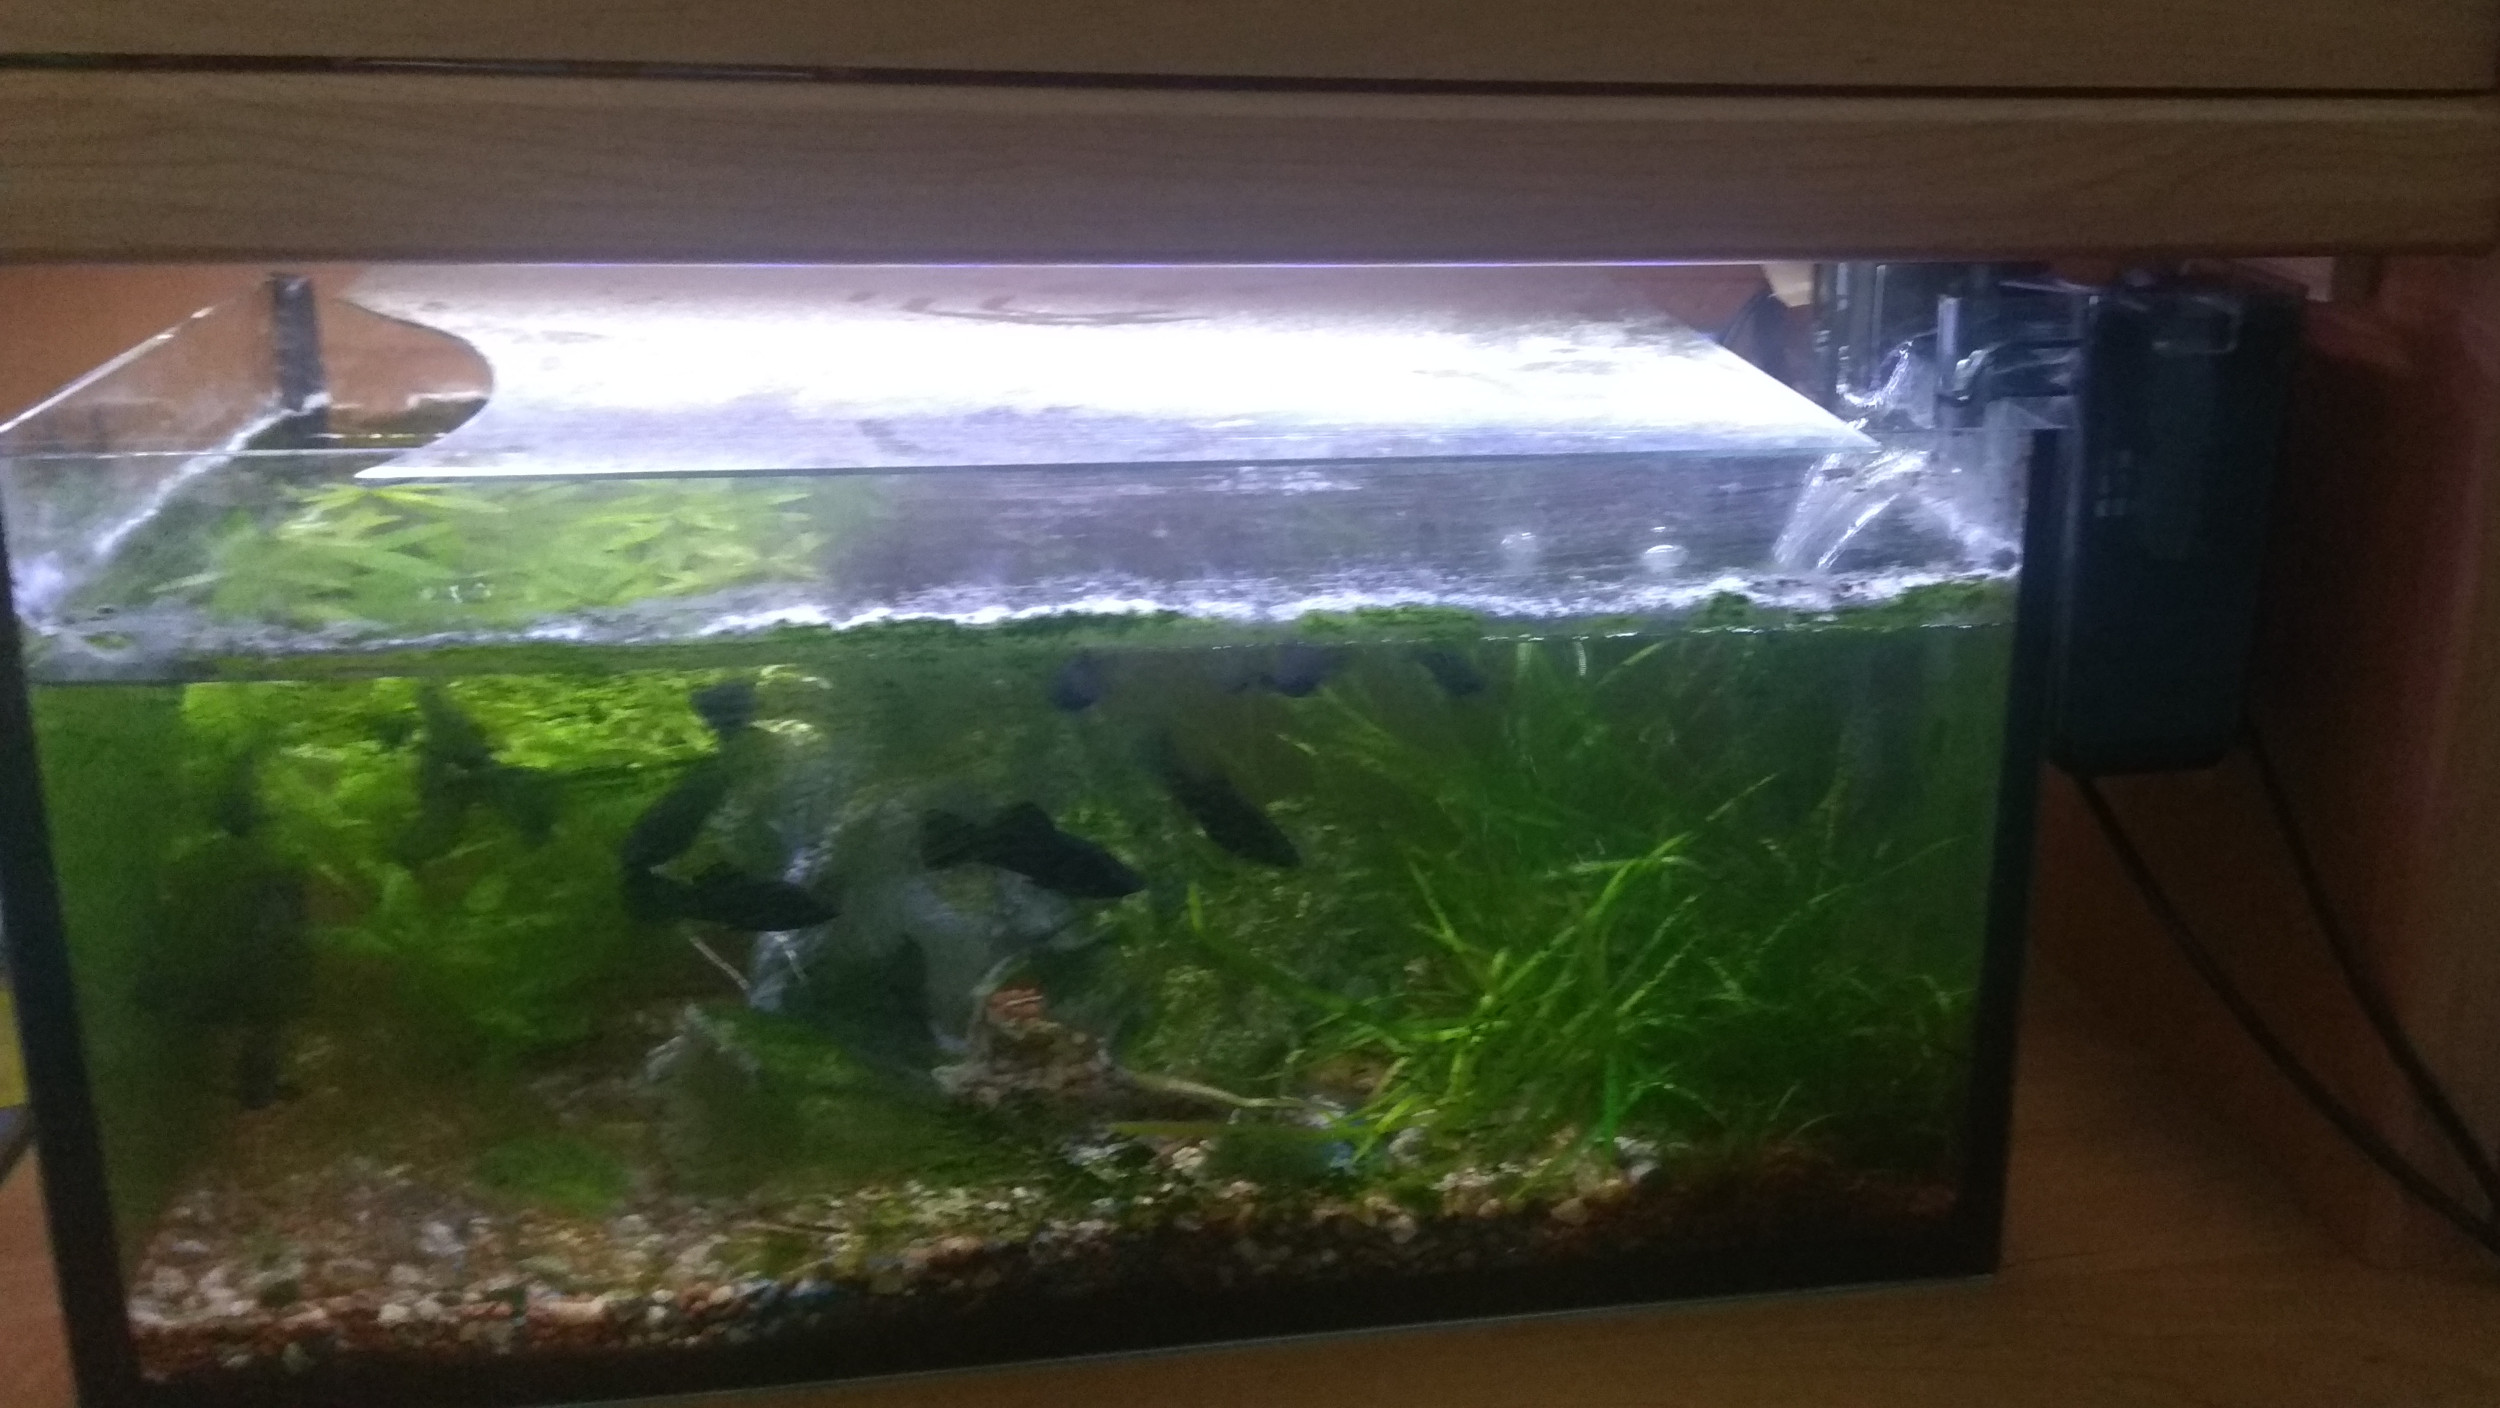
\includegraphics[width=0.8\textwidth]{akvarko.jpg}
		\caption{Naše akvárium, souhrnné foto.}
		\label{fig:akvarko}
	\end{figure}

	\begin{figure}[!h]
		\centering
		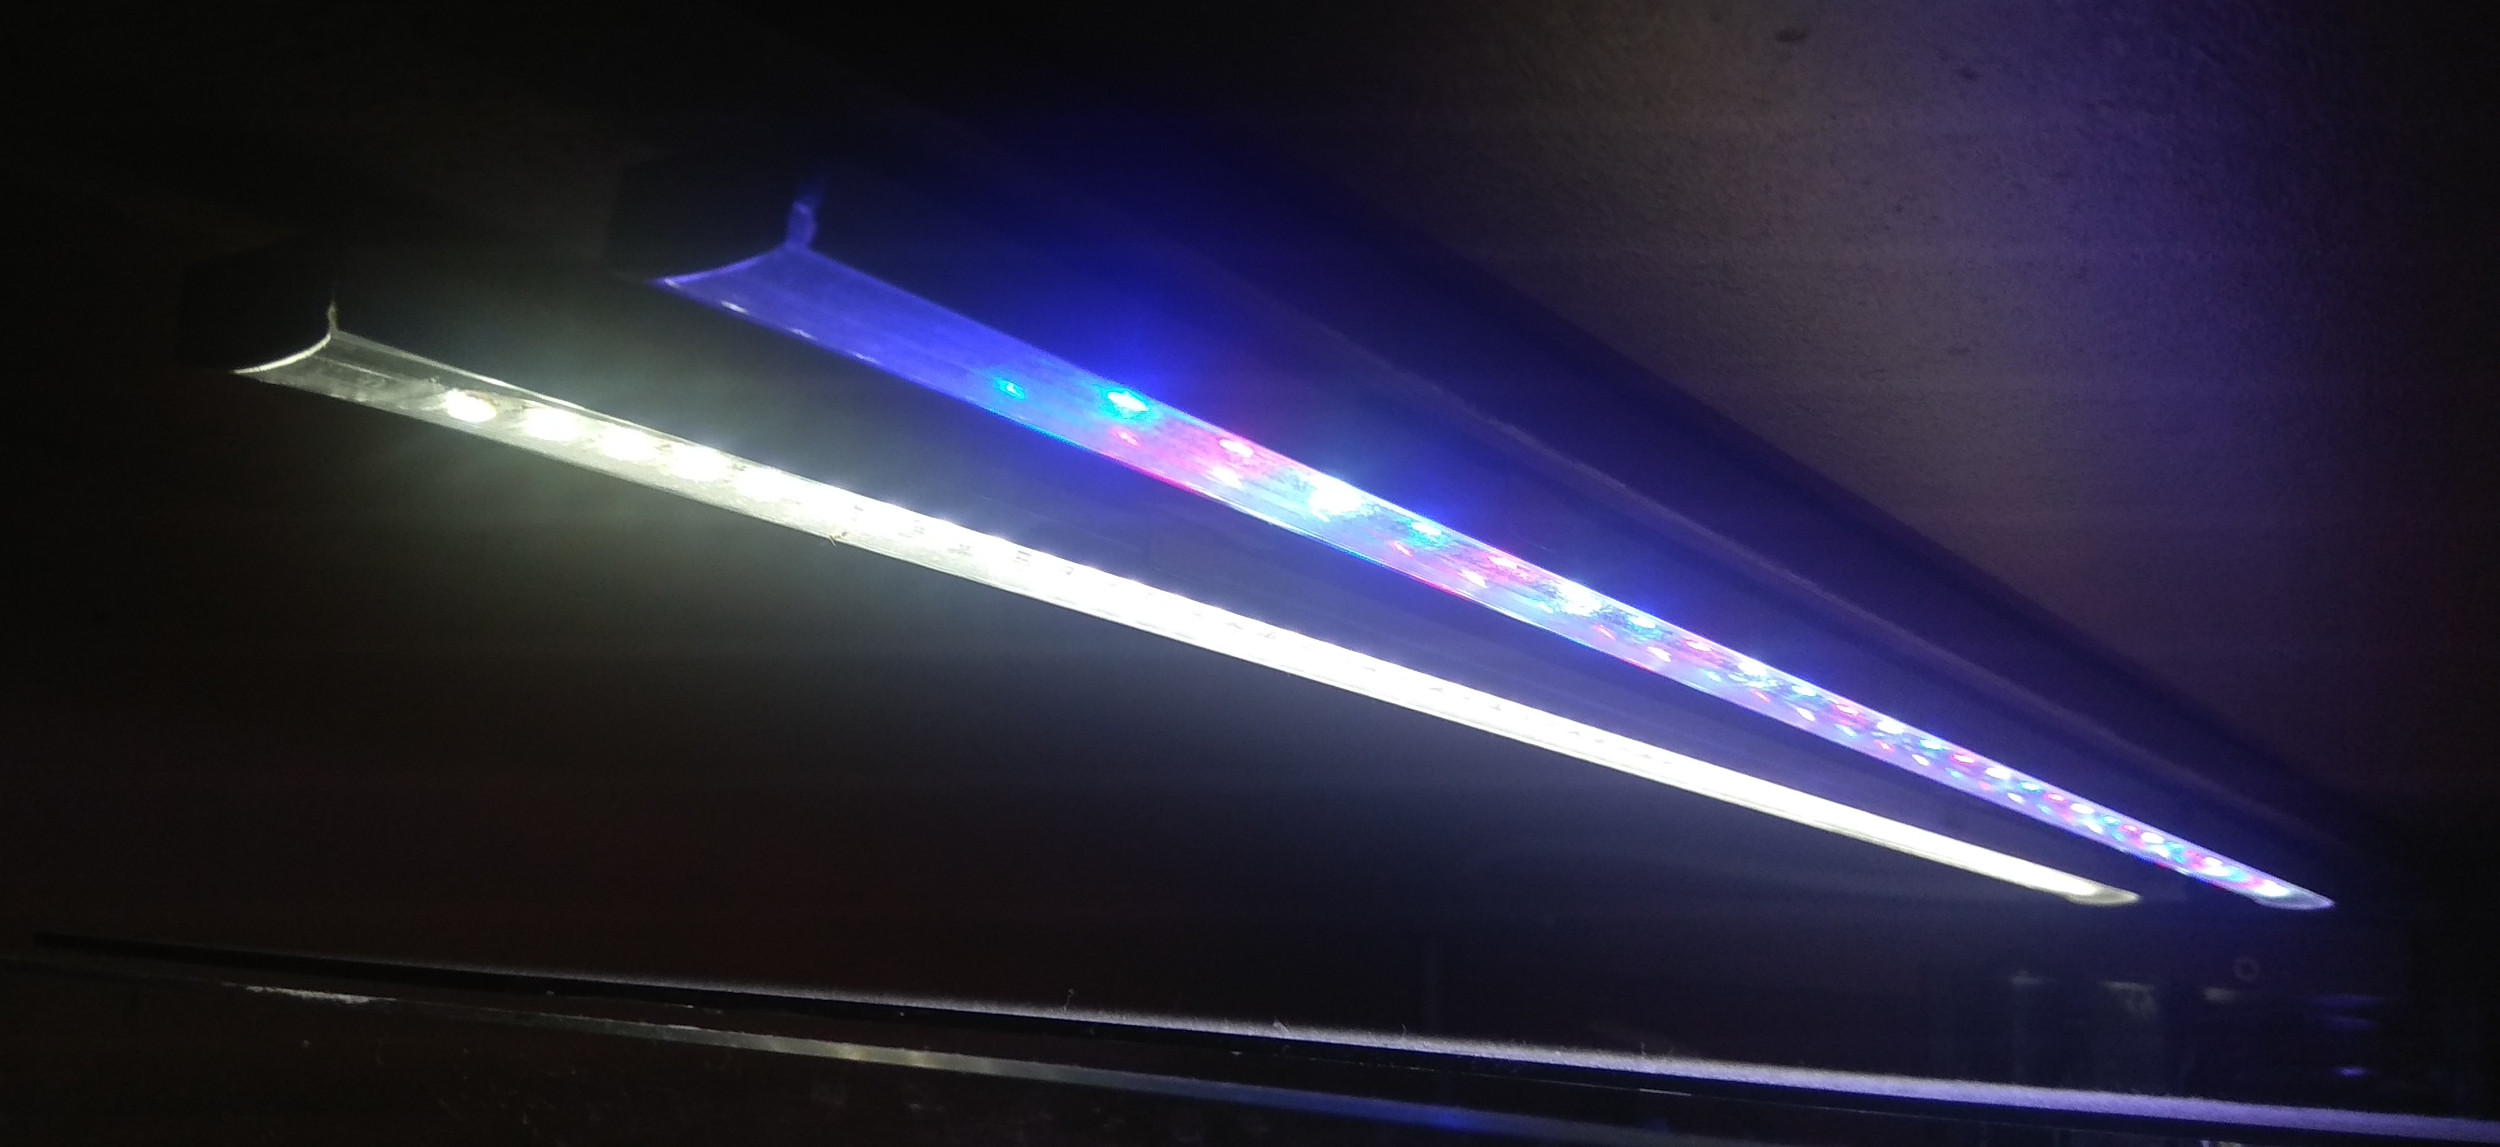
\includegraphics[width=0.8\textwidth]{svetla.jpg}
		\caption{Osvětlení formou dvou běžných LED pásků, ovládám každý zvlášť.}
		\label{fig:svetla}
	\end{figure}
	
	\begin{figure}[!h]
		\centering
		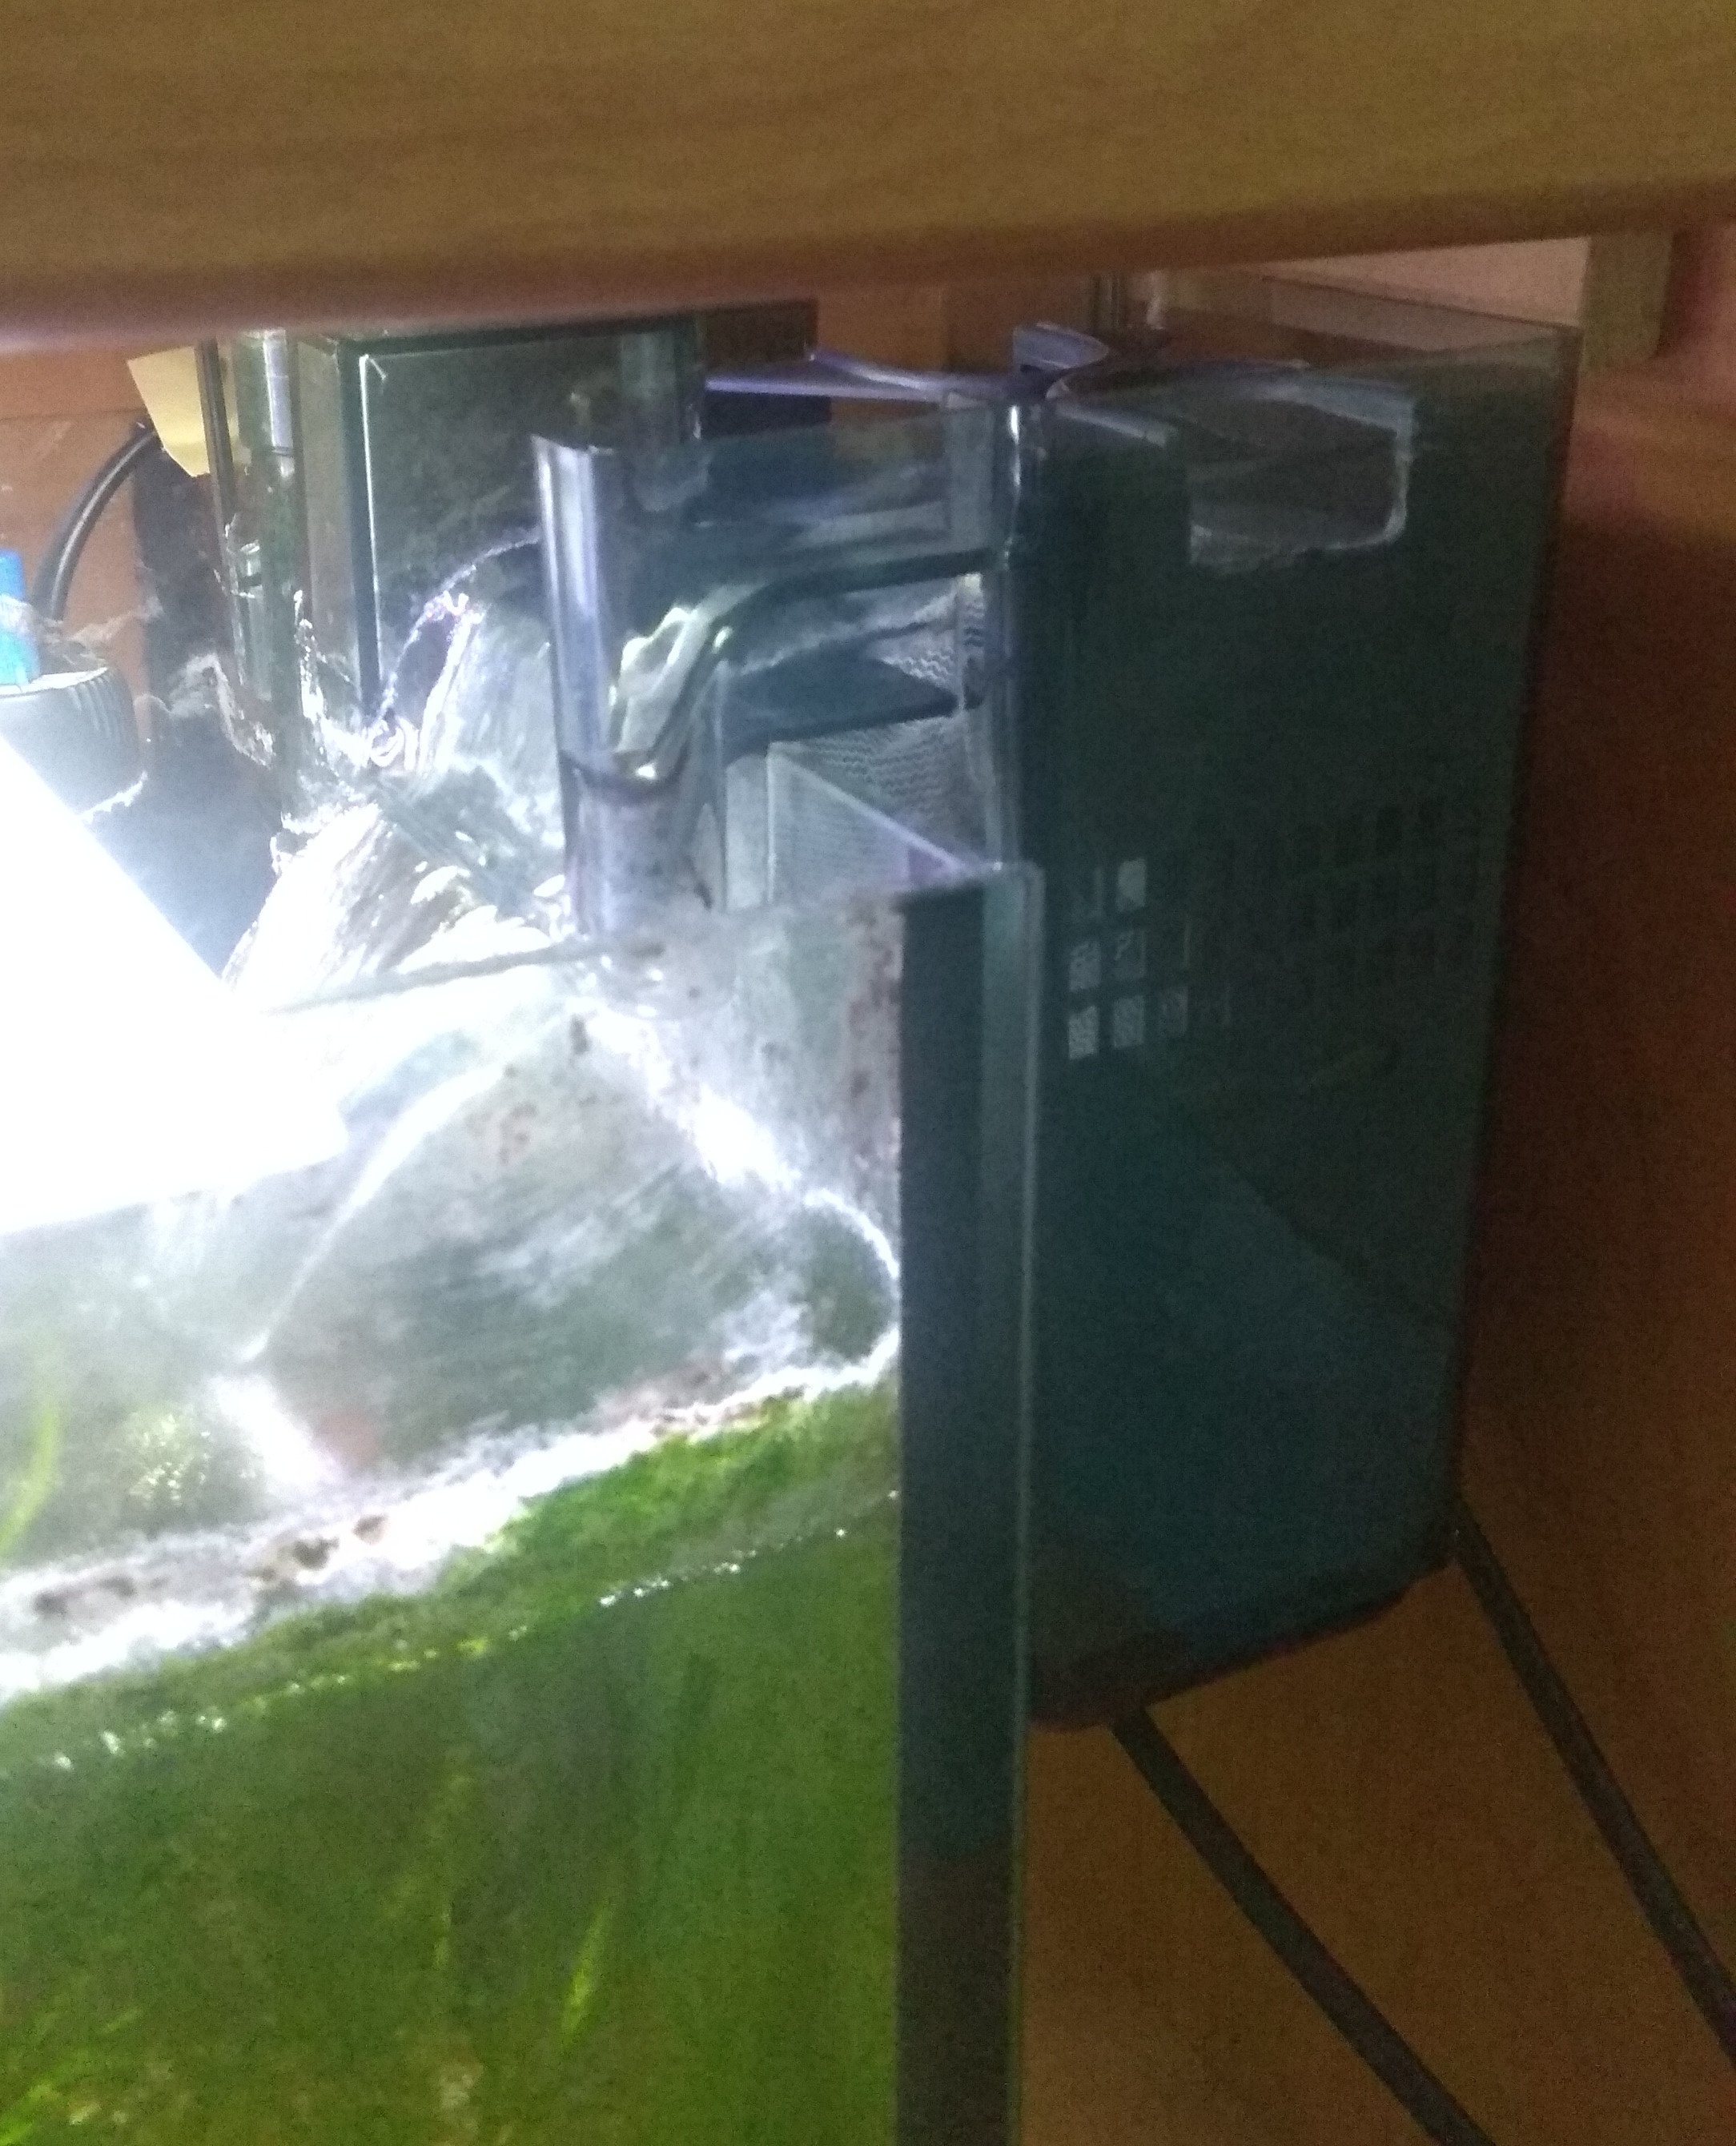
\includegraphics[width=0.6\textwidth]{filtr.jpg}
		\caption{Detail filtru.}
		\label{fig:filtr}
	\end{figure}

	\begin{figure}[!h]
		\centering
		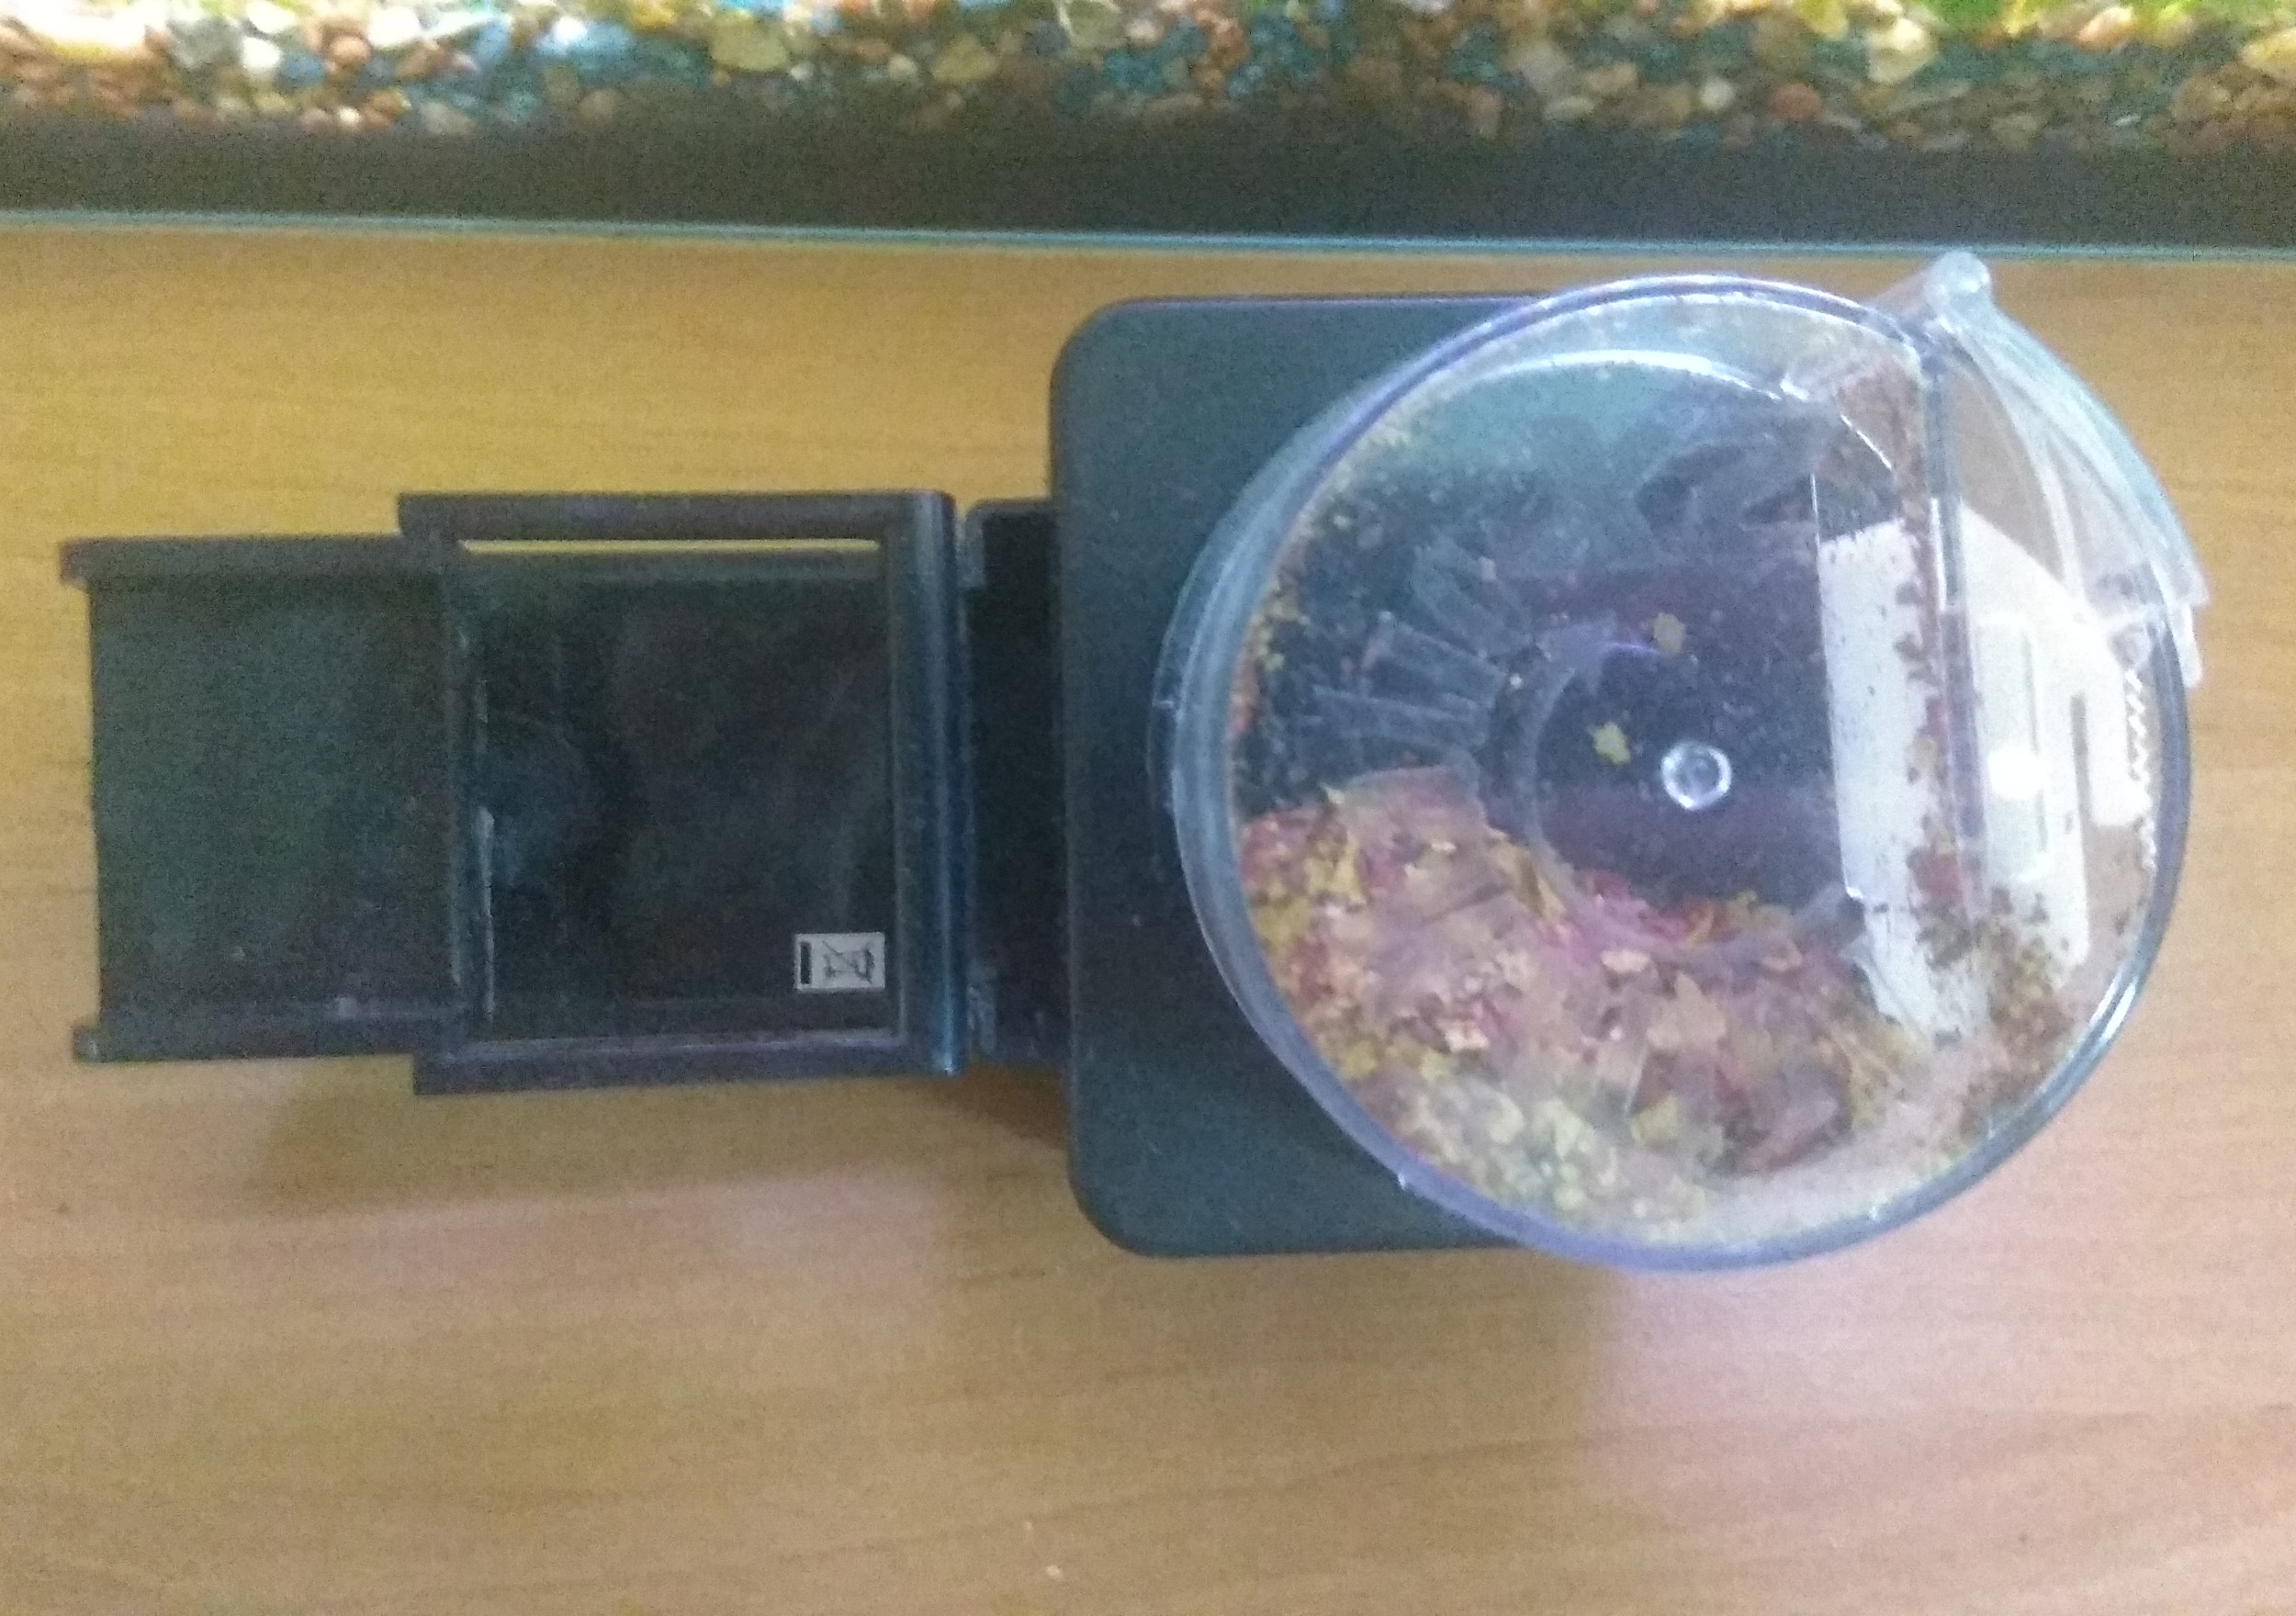
\includegraphics[width=0.8\textwidth]{krmitko.jpg}
		\caption{Automatické krmítko na baterie, rád bych nahradil vlastním řešením.}
		\label{fig:krmitko}
	\end{figure}


\clearpage
\section*{Popis verze Alpha :)}
	\begin{figure}[!h]
		\centering
		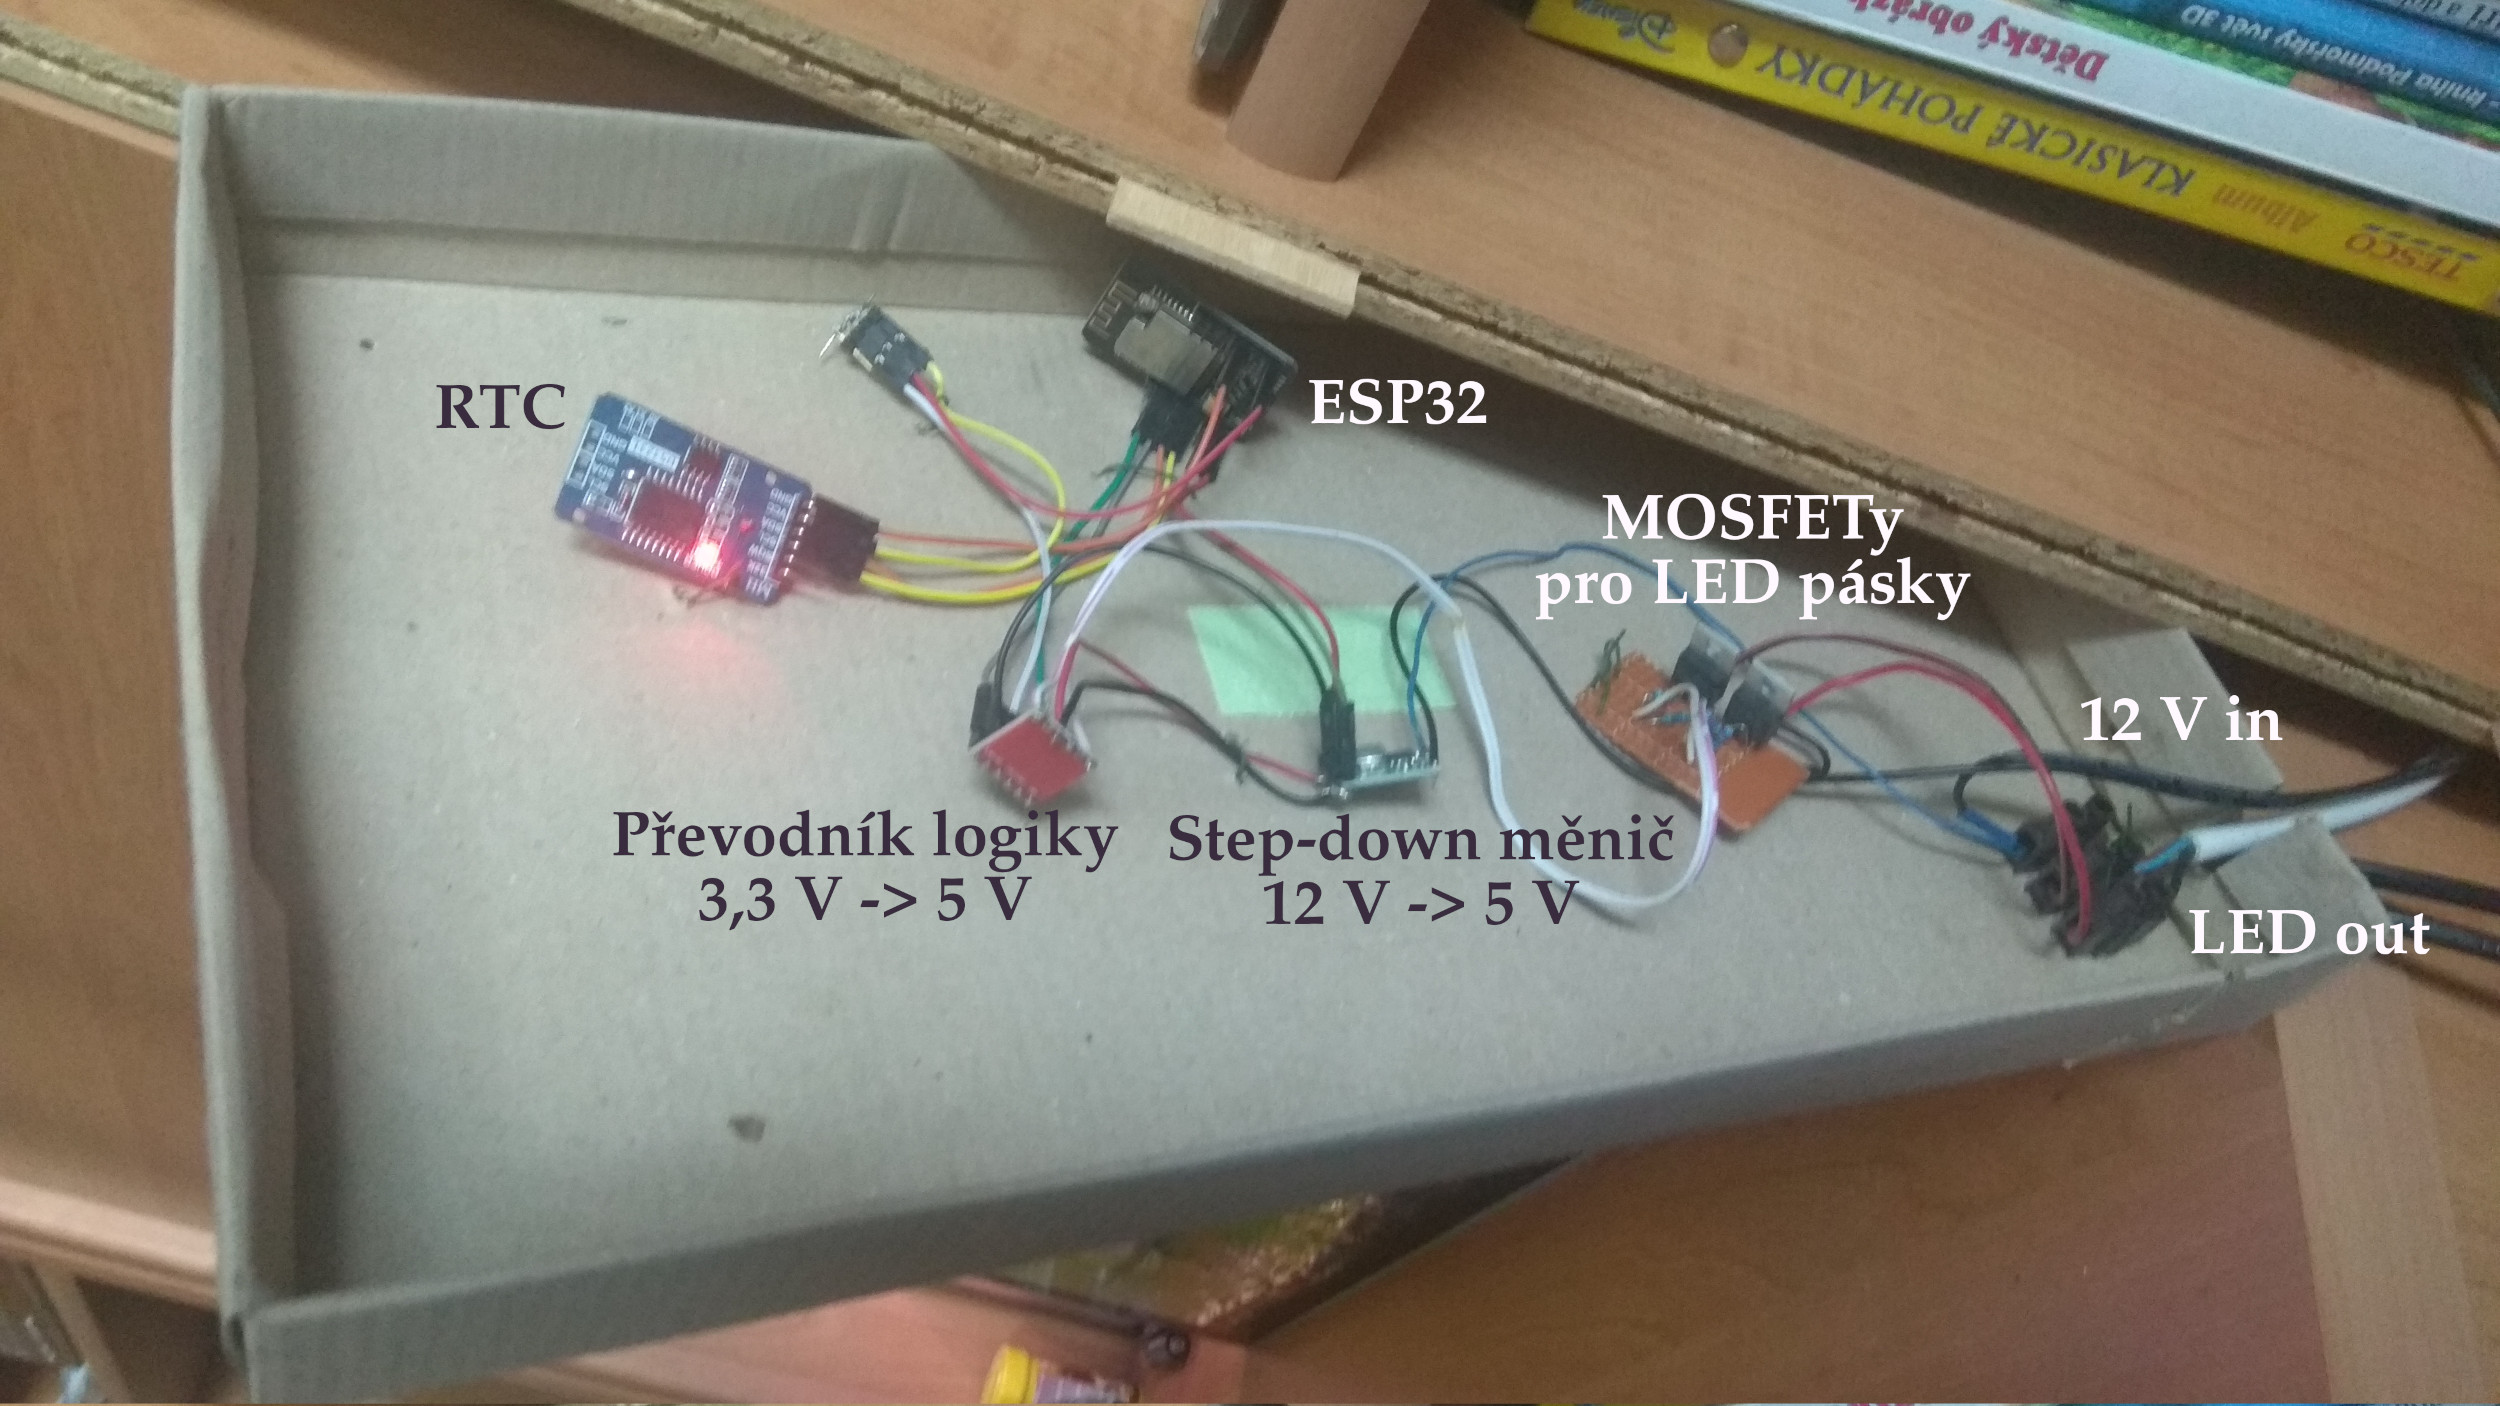
\includegraphics[width=0.9\textwidth]{moduly.jpg}
		\caption{moduly}
		\label{fig:moduly}
	\end{figure}
	Starší středoškolský projekt je vytvořený na úrovni modulů, je použit kontroler ESP32, na kterém běží webserver. Zařízení slouží pouze k ovládání světel, přes webovou stránku lze nastavit čas a rychlost rozsvícení a zhasnutí. 
	
	Kód je psán v Arduino frameworku, což byla v danou chvíli rozumná volba, ale teď bych se mu rád pokusil vyhnout. 
	Pro ovládání světel (LED pásky) jsem použil mosfet tranzistory řízené PWM pinem, také nebyly zvoleny vhodně, musel jsem použít předovník úrovně z \qty{3.3}{\volt} na \qty{5}{\volt}, aby bylo možné tranzistor plně otevřít.

	Za běžných podmínek zařízení funguje, ale například po výpadku elektřiny často končí v bootovací smyčce a je potřeba ručně zmáčknout reset, na stabilitu bych se tedy taky rád zaměřil.
d


	\section*{Senzory}
	Jednou variantou je připojení každého senzoru zvlášť na konkrétní místo s tím, že doplňující obvody (pull-up / pull-down rezistory, kapacitory, ...) budou přímo na hlavní DPS, toto řešení je ale málo flexibilní a hrozí chybné zapojení uživatelem.

	Lepším řešením by byl univerzální konektor pro všechny senzory, doplňující součástky pak musejí být přímo v modulu senzoru společně s velmi málo náročným mikrokontrolerem tak, aby všechny senzory z pohledu hlavního zařízení využívaly stejný komunikační protokol. Tento systém mi přijde také mnohem lépe rozšiřitelný.
	
	Senzory, které chci vytvořit:
	\begin{itemize}
		\item Teploměr
		\item Výška hladiny vody
		\item Kontrola průtoku vody filtrem (ještě potřeba promyslet)
		\item Volitelně: Osvětlení, PH, další parametry vody
	\end{itemize}


	\section*{Existující řešení}
	\subsection*{Komerční řešení}
	\begin{itemize}
		\item GHL
		\begin{itemize}
			\item Komplexní, asi nejlepší na trhu.
			\item Cena setu až ke 30 000 Kč.
		\end{itemize}

		\item Neptune Systems - Apex
		\begin{itemize}
			\item Komplexní, také jeden ze špičky na trhu.
			\item Cena setu přes 20 000 Kč.
		\end{itemize}
		
		\item Hydros
		\begin{itemize}
			\item Komplexní, modulární systém.
			\item Cena setu do 10 000 Kč, ale je méně obsáhlý.
		\end{itemize}

		\item Seneye
		\begin{itemize}
			\item Pouze monitoring
		\end{itemize}

		\item Jednotlivé jednoúčelové produkty (samostatné ovládání světel, krmení, ...)
		\begin{itemize}
			\item Pro menší domácí akvária, nižší cena, ale komplikované nastavení 
		\end{itemize}
	\end{itemize}
	
	\subsection*{DIY řešení}
	\begin{itemize}
		\item Vzorová diplomka -- akvarium
		\item Pěkně zpracovaný kontroler pro terárium
		\begin{itemize}
			\item \url{https://brushknight.medium.com/terrarium-controller-idea-%EF%B8%8F-v1-4-b8ee96cfbd22}
		\end{itemize}
	\end{itemize}


	\section*{Plán práce}
	\begin{enumerate}
		\item Průzkum trhu a existujících řešení
		\item Volba konkrétních senzorů
		\begin{enumerate}
			\item Test různých typů
			\item Volba komunikačního protokolu
			\item Na breadboardu, nejlépe už základní kód v ESP IDF
		\end{enumerate}
		\item Seznámení s ESP IDF
		\item Vyřešení ovládání světel  -- volba vhodných MOSFETů + test
		\item Ovládání periferií 230V -- rozhodnutí smart plug vs svorkovnice
		\item Návrh schématu s devkitem
		\item Prototyp s devkitem -- test
		\item Schéma bez devkitu, layout DPS
		\item Objednání DPS, osazení, test 
		\item (Oprava chyb, možná nová DPS) -- možné opakování tohoto kroku
		\item firmware + řídící software
		\item Test v provozu 
	\end{enumerate}

\end{document}

